% 原书印刷79--85页，PDF物理106--112页，完整章末.
\subsection{讨论}\label{sec:2.5}

\subsubsection{直方图均衡化}\label{sec:2.5.1}

图像处理中遇到单调运输映射的一个十分典型的问题是\emph{直方图均衡化}（histogram equalization）. 问题背景很容易说明：取一张黑白数字图像，考虑所有可能的灰度级；这些灰度级编号为$0$至$255$；对每个$i=0,\ldots,255$，统计恰好具有该灰度级的像素数，并绘制直方图. 在某些情形下，我们希望将给定图像变成另一张仍表示同一主体、却具有不同直方图的图像. 为什么？典型例子如下：有两张图像A和B，它们应当表示同一物体在不同时刻的情形，只有细微变化（某些东西移动了）；想要比较它们，但B碰巧比A暗得多（这意味着B的直方图比A的更集中于图的右侧）. 因而在比较之前，通常希望将B变成新图像B$'$，使B$'$的明暗水平与A可比，也就是使B$'$的直方图等于A的直方图. 类似地，也可以考虑A与B表示同一物体的两个部分，需要将两张图像拼合的情形，但两张局部图像可能从不同角度拍摄，光照也不同.

另一些情形中，只有一张图像，但其直方图过分集中于某个峰附近. 这意味着像素具有不同灰度级，但差异不大. 为更清楚地看出图像中的内容，希望增强对比度，这对应于使用分布更广的直方图. 此时可指定目标直方图，例如均匀直方图，其中每个灰度级由相同数量的像素使用. 从不过分集中在同一灰度级附近、从而不浪费信息的意义上说，这是最好的直方图.

在所有这些情形中，希望所作变换按灰度级起作用，而非逐个像素起作用：寻找从灰度级集合$X$到自身的映射$\mathrm T$（所有灰度级为$x$的像素都变为灰度级$\mathrm T(x)$），并指定变换后图像的直方图. 这等价于说，$X$上有一个测度$\mu$，希望施加形如$\mathrm T_\#\mu=\nu$的条件. 这里重要的是，空间$X$是$\mathbb R$的子集，即一维且有序. 对$\mathrm T$的自然要求是单调递增. 这一要求表达了不希望将较暗与较亮像素的次序颠倒.

除了在这一离散背景下（灰度级只在有限整数集中取值），两个测度$\mu$与$\nu$均有原子（因而运输映射可能不存在）这一点外，情形恰好就是本章描述的情形. 实际中，运输映射不存在的问题可以用几种方法解决：可以引入舍入规则，或使用运输方案；后者对应于让原图中颜色相同的像素使用不同颜色，也就是分裂质量.

对于彩色图像，情形更复杂. 此时颜色空间$X$变为三维，单调运输的概念不再有意义. 显然，二次最优运输（Brenier映射）可扮演单调映射的角色，因为它满足向量意义的单调性
$(\mathrm T(x)-\mathrm T(y))\cdot(x-y)\ge0$. 另一方面，它的计算代价高（\autoref{sec:6}将介绍计算它的若干数值方法及相应困难），而且它的某些特点可能对这类图像处理应用没有用处（例如，它是一个梯度）.

目前正在研究几种解决办法：寻找更正则、但与最优映射差别不太大的运输映射\cite{b163}，或通过若干一维构件的复合、叠加来产生映射，使之保留某些单调性且更容易计算（见\cite{b252}与\autoref{sec:2.5.2}）.

此外，有时颜色空间的各分量并非同等重要，可以决定只看其中一个或两个分量，或将它们分别处理. 此时，颜色经常用不同的参数组描述.

例如，\cite{b140}对颜色空间的色调分量提出了圆周上一维分析的一些应用（使用分为色调、饱和度与明度的HSL分解）.

同一颜色空间也可写成一维信息与二维信息的组合：前者是亮度信号（luma），对应于R、G、B三个分量的加权平均，表示图像的亮度；后者称为色度（chrominance或chroma），表示颜色信息. \autoref{fig:2.4}给出一维与二维最优运输的一个应用，在颜色十分不同的两条街道图像之间进行颜色迁移.

关于一维直方图均衡化及三维颜色迁移与最优运输之间联系的更广泛讨论，参见\cite{b163,b255}及其中的参考文献（特别是\cite{b242,b259}等较早的论文）.

\begin{figure}[htbp]
\centering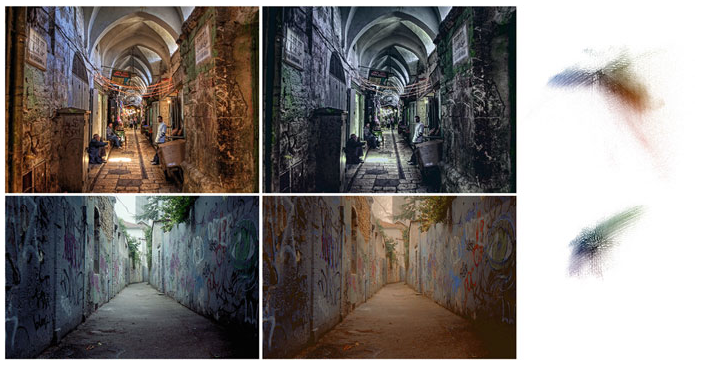
\includegraphics[width=\linewidth]{assets/ch02-fig-2-4.pdf}
\caption{第一列：不同光照下的露天市场拱廊与一条墙上有涂鸦的西方狭窄街道. 第二列：两张图像分别采用另一张的颜色. 第三列：它们的色度直方图（采用CIE-lab表示）. 迁移分别独立地作用于一维亮度特征与二维色度特征. 图中只显示色度直方图. 图片由G.~Peyré惠予提供.}\label{fig:2.4}
\end{figure}

\subsubsection{由一维构造得到高效单调映射}\label{sec:2.5.2}

在许多应用中，特别是图像处理（如上一小节\autoref{sec:2.5.1}），人们尝试构造“好的”运输映射. 它们不一定最优，但至少满足两个标准：计算上容易求出，并具有某些“单调性”. 同时满足这两项要求的一个好办法，是利用一维构件来构造这些映射.

最先想到的可能是使用Knothe映射. 然而，这一选择的主要缺点是高度各向异性. 标准正交基的选择至关重要，而且映射赋予不同坐标轴的作用很不相同.

文献\cite{b252}包含另一种想法，提出了所谓\emph{迭代分布迁移算法}（Iterative Distribution Transfer algorithm）：给定源测度$\mu$与目标测度$\nu$；从$\mu_0=\mu$出发，作者递归构造一列映射$\mathrm T_n$，并令$\mu_{n+1}=(\mathrm T_n)_\#\mu_n$. 构造这一序列的目的是使$\mu_n$收敛到$\nu$；这意味着，对足够大的$n$，映射$\mathrm T_n\circ\mathrm T_{n-1}\circ\cdots\circ\mathrm T_1\circ\mathrm T_0$把$\mu$运输到一个十分接近$\nu$的测度$\mu_n$.

在\cite{b252}的构造中，映射$\mathrm T_n$如下得到：每一步$n$随机选择一个标准正交基$B_n$；然后将$\mathrm T_n^j$定义为从$(\pi_j)_\#\mu_n$到$(\pi_j)_\#\nu$的单调运输映射，其中$\pi_j$为所选基第$j$个坐标上的投影；在相应基中，令
$\mathrm T_n(x)=(\mathrm T_n^1(x_1),\ldots,\mathrm T_n^d(x_d))$.

这一选择背后有两个想法：首先，所有映射$\mathrm T_n$都容易计算，由有限多个一维单调映射组成，并具有单调性；其次，若以适当多样的方式选择基$B_n$，算法停留于一个不再改变的测度$\mu_n$的唯一可能，是$\mu_n$与$\nu$在所有方向上具有相同投影. 根据\autoref{box:2.4}中关于Radon变换与X射线变换的讨论，这蕴含$\mu_n=\nu$，而且显然提示$\mu_n$的极限应为$\nu$.

然而，这种收敛虽在经验中被观察到，\cite{b252}却只在$\nu$为Gauss测度、且基$B_n$为在标准正交基集合上均匀分布的独立同分布随机变量时证明了它. 修订后更一般的证明还可参阅\cite{b65}第5章.

\begin{sourcebox}{相关知识：Radon变换与X射线变换}\label{box:2.4}
\begin{definition*}
给定$\mathbb R^d$上的测度$\mu$，将$\mu$的\emph{Radon变换}$R\mu$定义为以$e\in\mathbb S^{d-1}$为参数的测度族$(\mu_e)$，其中$\mu_e=(\pi_e)_\#\mu$，$\pi_e(x):=x\cdot e$. 当$\mu$绝对连续时，这些测度也绝对连续；通过$R\mu(e,t)=f_e(t)$与$\mu_e=f_e(t)\,dt$，可将$R\mu$定义为$\mathbb S^{d-1}\times\mathbb R$上的函数. 在$d>2$维，可以考虑到超平面而非直线的投影（注意，投影到所有$d-1$维超平面，意味着考虑测度或其密度在任意一维直线上的积分）. 这种变换称为\emph{X射线变换}（X-ray transform），但$d=2$时Radon变换与X射线变换相同. 更多细节和应用例如见\cite{b192}.
\end{definition*}

\begin{proposition*}
给定$\mathbb R^d$上的两个测度$\mu,\nu$，若它们的Radon变换相同，则$\mu=\nu$.
\end{proposition*}
\begin{proof}
注意，$\int_{\mathbb R^d}e^{i\xi\cdot x}\,d\mu=\int_{\mathbb R}e^{it|\xi|}\,d\mu_{\xi/|\xi|}(t)\,dt$. 这意味着Radon变换唯一确定测度的Fourier变换，故$R\mu=R\nu\Rightarrow\widehat\mu=\widehat\nu$. 由Fourier变换的标准结果，得到$\mu=\nu$.
\end{proof}

Radon变换与X射线变换是断层成像等应用中十分知名的对象. 医学图像中的计算机断层扫描设备正是基于X射线变换的求逆.
\end{sourcebox}

关于构造类似运输映射的另一种有趣想法来自M.~Bernot. 它的许多特点与\cite{b252}的方法相同.

考虑两个测度$\mu,\nu\in\mathscr P(\mathbb R^d)$，将它们投影到任意一维方向. 对每个$e\in\mathbb S^{d-1}$（$\mathbb R^d$的单位球面），取由$\pi_e(x)=x\cdot e$给出的映射$\pi_e:\mathbb R^d\to\mathbb R$，考虑像测度$(\pi_e)_\#\mu$与$(\pi_e)_\#\nu$. 它们仍为实直线上的测度，将它们之间的单调最优运输记为$\mathrm T_e:\mathbb R\to\mathbb R$. 想法是，就方向$e$而言，$\mathbb R^d$中每个点$x$都应位移一个向量
$S_e(x):=(\mathrm T_e(\pi_e(x))-\pi_e(x))e$. 为作整体位移，考虑
\[
S(x)=\fint_{\mathbb S^{d-1}}S_e(x)\,d\mathscr H^{d-1}(e),
\]
其中$\mathscr H^{d-1}$为球面上的均匀测度.

同样，没有理由保证$\mathrm{id}+S$是从$\mu$到$\nu$的运输映射. 但若固定一个较小的时间步长$\tau>0$，使用位移$\tau S$得到测度$\mu_1=(\mathrm{id}+\tau S)_\#\mu$，便可以像\cite{b252}那样迭代这一构造，只是运输映射$\mathrm T_n$的定义不同. 同样，预期这样构造的测度序列$\mu_n$收敛到$\nu$，但问题尚未真正解决. 从经验角度看，以此方式得到的运输映射相当令人满意，尤其已在离散情形中检验过（有限多个质量相等的Dirac质量，即所谓\emph{指派问题}）. \autoref{fig:2.5}给出一个例子，比较通过线性规划方法（见\autoref{sec:6.4.1}）得到的最优运输，以及M.~Bernot通过这些一维切片思想得到的指派.

\begin{figure}[htbp]
\centering
\includegraphics[width=\linewidth]{assets/ch02-fig-2-5.pdf}
\caption{环带与鸭子上有限个点之间的最优运输. 颜色表示从环带上的点到鸭子上的点的指派. 中图为一维切片指派；右图为二次成本的最优映射. 两种结果非常相似（但能找到少数颜色不同的点，表示指派略有不同）. 图片经许可取自\cite{b256}.}\label{fig:2.5}
\end{figure}

此外，\autoref{sec:5.5}将看到，这种想法还可以在概率测度集合上构造一种有趣的距离（将逐个方向定义的距离取平均：它比相应的多维距离容易计算得多）. 在\autoref{sec:8.4}还将说明，上述迭代算法确实对应于一种梯度流演化.

\subsubsection{通过Knothe或Brenier映射证明等周不等式}\label{sec:2.5.3}

本章最后一个讨论小节回顾最优运输最引人注目的应用之一，即它在几何不等式中的作用. 这里将看到，既可使用最优（Brenier）映射，也可使用Knothe映射来证明等周不等式.

有趣的是，处理几何不等式确实是使用Knothe运输最初的动机之一（见\cite{b203}）. 不过，下面这一等周不等式的简短证明最初由Gromov发现（见\cite{b236}的附录），而Knothe在\cite{b203}中的最初目标是建立有关凸集的其他不等式.

等周不等式说，每个集合$E$的周长都不小于具有相同体积$|B|=|E|$的球$B$的周长. 利用体积与周长的缩放性质，可以将这一事实写成
\[
\operatorname{Per}(E)\ge d\omega_d^{1/d}|E|^{1-1/d},
\]
其中$\omega_d$为$\mathbb R^d$中单位球的体积.

与这些讨论小节中的惯例一样，不会完整交代所提想法的细节，对正则性的处理也相当粗略. 无论如何，可将$E$看作$\mathbb R^d$中的光滑区域. 通过缩放，还可假设$E$与单位球$B=B(0,1)$具有相同体积.

证明这一结果的想法如下：考虑密度$\mu=\mathscr L_E$与$\nu=\mathscr L_B$，使用这两个密度之间的Knothe运输，记为$\mathrm T$. 由前面对$\mathrm T$的Jacobi矩阵的讨论，它仅有正特征值，且满足
\[
\det(D\mathrm T)=\frac{|B|}{|E|}=1
\]
（行列式上不取绝对值）. 因此可以写成
\begin{equation}\label{eq:2.8}
\omega_d=|B|=|E|=\int_E(\det(D\mathrm T))^{1/d}
\le\frac1d\int_E\nabla\cdot\mathrm T
=\frac1d\int_{\partial E}\mathrm T\cdot\mathbf n
\le\frac1d\operatorname{Per}(E),
\end{equation}
其中的不等式分别来自对$D\mathrm T$的特征值使用算术--几何平均不等式
$\frac1d\sum_i\lambda_i\ge(\lambda_1\cdots\lambda_d)^{1/d}$（给出行列式与迹之间的不等式，迹即$\mathrm T$的散度），以及$\mathrm T$取值于$B$这一事实，从而$\mathrm T\cdot\mathbf n\le1$. 这就证明了$\operatorname{Per}(E)\ge d\omega_d=\operatorname{Per}(B)$.

\begin{center}
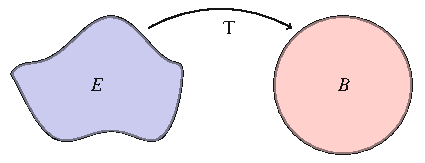
\includegraphics[width=.62\linewidth]{assets/ch02-isoperimetric.pdf}
\end{center}

注意，我们只使用了$\mathrm T$的Jacobi矩阵具有正特征值、以及它把一个测度运输到另一个测度这两个事实. Brenier映射也满足这些性质，只是在首次完成这一证明时，还不知道这个映射.

同一证明也可用于证明最优集合的唯一性（即若集合$E$与单位球具有相同体积，且$\operatorname{Per}(E)=d\omega_d$，那么忽略零测集后，它就是一个单位球）.

使用Brenier映射会大大简化等号情形的研究. 事实上，假设上述不等式均取等号：这意味着几乎处处有$(\det(D\mathrm T))^{1/d}=(\nabla\cdot\mathrm T)/d$；由算术--几何平均不等式的等号情形，得到$D\mathrm T$的特征值必须全都相等. 再由行列式条件，它们都等于$1$. 若还知道矩阵对称（Brenier映射如此，而Knothe映射不然），则得到$D\mathrm T=\mathrm I$与$\mathrm T(x)=x+x_0$. 因为$\mathrm T$是平移，便得到在相差一个平移的意义下$E=B$.

对Knothe运输稍困难一些，因为$D\mathrm T$不对称. 不过，若所有特征值都为$1$，可推出最后一个分量$\mathrm T^d$是平移. 若一开始就假设（允许先作固定平移）$E$与$B$具有相同重心，则这一平移是恒等映射. 这意味着$(\pi_d)_\#\mu=(\pi_d)_\#\nu$. 这还不足以得到$\mu=\nu$，从而得到$E=B$；但可使用Knothe运输不具有各向同性（即其定义依赖于坐标轴的选择）、且坐标轴方向任意这一事实. 因而，若集合$E$使等周不等式取等号，则它在任意方向上的投影都与球的投影相同. 这蕴含$E\subset B$，再由体积相等得到$E=B$（也可通过测度和Radon变换的概念论证，因为对第$d$根坐标轴的任意方向均有$(\pi_d)_\#\mu=(\pi_d)_\#\nu$，就蕴含$\mu=\nu$）.

最后强调，等周不等式显然可用许多其他方法证明，但最近一个深入的加强结果，即各向异性等周不等式的定量版本（其中周长的定义改变，最优集合不再是球，而是另一凸集，即另一范数的单位球），却只有借助最优运输技巧才以最优指数得到证明（见\cite{b167}及简短综述\cite{b276}）.
